\documentclass[border=10pt]{standalone}
\usepackage{tikz}
\usetikzlibrary{arrows.meta,calc}

\begin{document}
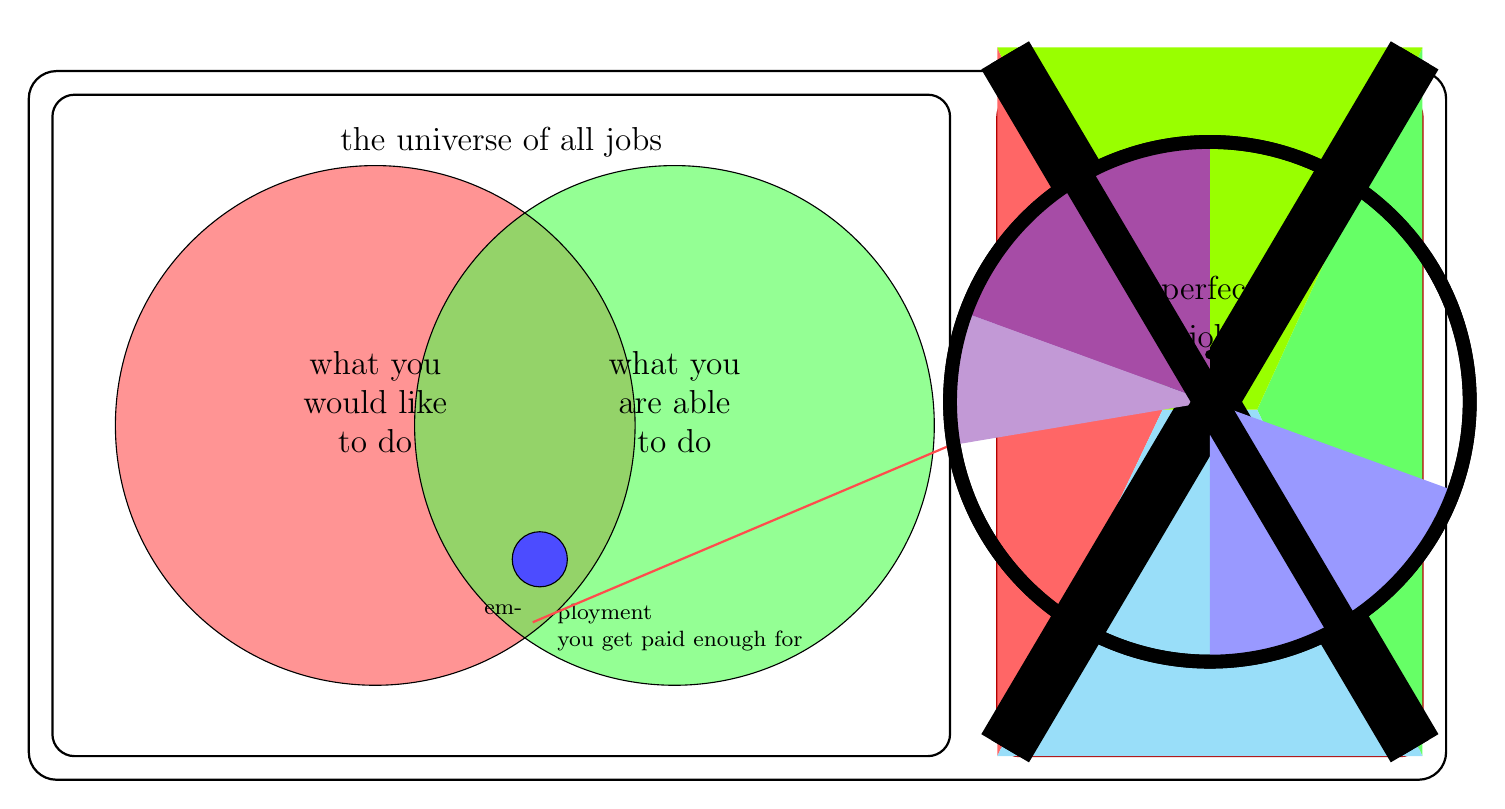
\begin{tikzpicture}[font=\sffamily]

% Global frame
\draw[rounded corners=10pt,thick] (0,0) rectangle (18,9);

% Left and right panel frames
\draw[rounded corners=8pt,thick] (0.3,0.3) rectangle (11.7,8.7);
\draw[rounded corners=8pt,thick,red!70!black] (12.3,0.3) rectangle (17.7,8.7);

% Title
\node[font=\large] at (6,8.1) {the universe of all jobs};

% --- Left Venn diagram -------------------------------------------------
\begin{scope}[shift={(1.2,1.1)}]
  % circle centers
  \def\R{3.3}
  \coordinate (L) at (3.2,3.4);
  \coordinate (R) at (7.0,3.4);

  % circles
  \fill[red!70,opacity=.6] (L) circle (\R);
  \fill[green!70,opacity=.6] (R) circle (\R);
  \draw (L) circle (\R);
  \draw (R) circle (\R);

  % labels
  \node[align=center,font=\large] at ($(L)+(0,0.3)$)
    {what you\\would like\\to do};
  \node[align=center,font=\large] at ($(R)+(0,0.3)$)
    {what you\\are able\\to do};

  % small employment circle
  \coordinate (E) at ($(L)!0.55!(R)+(0,-1.7)$);
  \fill[blue!70] (E) circle (0.35);
  \draw (E) circle (0.35);

  % employment text
  \node[anchor=north east,align=right,font=\footnotesize] at ($(E)+(-0.1,-0.45)$)
      {em-};
  \node[anchor=north west,align=left,font=\footnotesize] at ($(E)+(0.1,-0.45)$)
      {ployment\\you get paid enough for};

\end{scope}

% Connecting zoom line
\draw[red!70,thick] (6.4,2.0) -- (12.3,4.5); % from small circle approx to right

% --- Right zoomed diagram ----------------------------------------------
\begin{scope}[shift={(12.3,0.3)}]
  % background coloured quadrants
  \fill[red!60] (0,0) -- (2.1,4.4) -- (0,9) -- cycle;           % left
  \fill[green!60] (5.4,9) -- (3.3,4.4) -- (5.4,0) -- cycle;     % right
  \fill[cyan!40] (0,0) -- (5.4,0) -- (3.3,4.4) -- (2.1,4.4) -- cycle; % bottom
  \fill[green!40!yellow] (0,9) -- (5.4,9) -- (3.3,4.4) -- (2.1,4.4) -- cycle; % top

  % big circle
  \coordinate (C) at (2.7,4.5);
  \def\RR{3.3}
  \draw[line width=5pt] (C) circle (\RR);

  % thick cross bands (diagonals)
  \draw[line width=20pt] (0.1,8.9) -- (5.3,0.1);
  \draw[line width=20pt] (0.1,0.1) -- (5.3,8.9);

  % clipped circle with coloured wedges
  \begin{scope}
    \clip (C) circle (\RR);
    % four wedges following diagonals
    \fill[blue!60] (C) -- ++(160:4) -- ++(90:4) -- ++(-20:4) -- cycle; % top
    \fill[blue!40] (C) -- ++(-20:4) -- ++(-90:4) -- ++(-200:4) -- cycle; % right
    \fill[blue!20!violet!40] (C) -- ++(-200:4) -- ++(-90:4) -- ++(160:4) -- cycle; % bottom
    \fill[violet!70] (C) -- ++(160:4) -- ++(90:4) -- ++(-20:4) -- cycle; % left (overlap)
  \end{scope}

  % Re-draw circle and diagonals to keep strong borders
  \draw[line width=5pt] (C) circle (\RR);
  \draw[line width=12pt] (0.1,8.9) -- (5.3,0.1);
  \draw[line width=12pt] (0.1,0.1) -- (5.3,8.9);

  % perfect job label
  \node[font=\large] at ($(C)+(0,1.4)$) {perfect};
  \node[font=\large] at ($(C)+(0,0.8)$) {job};
  \fill ($(C)+(0,0.6)$) circle (0.06);

\end{scope}

\end{tikzpicture}
\end{document}